
\chapter{Exact Inference in Probabilistic Graphical Models}

In the context of inference, out task is, given a joint distribution $p(X) = p(x_1, \dots, x_n)$ to compute marginals or conditionals of the distribution.

We formalize this by considering two disjoint subsets of r.v.: $y \subseteq x, z \subseteq x$ s.t. $y \cap z = \emptyset$ and $y \cup z \subseteq x$.

Given that we observe $y$, we want to compute the conditional
$$
    \begin{array}{rl}
        p(z|y = \bar{y})
        & = \sum_{x}^{}p(z,x'|y = \bar{y}) discrete r.v. \\
        & = p(z|y = \bar{y} = \int_{x}^{}p(z,x'|y = \bar{y})) continuous r.v.
    \end{array}    
$$

being $x'$ s.t. $x' \cup y \cup z = x$.

\textbf{Remark:} this summation can be of the order of $O(\mathcal{K}^m)(|x'|=m)$, hence obtaining this marginalization is computationally challenging!

Our goal is to carry out this computation efficiently, by leverage the factorization implied by the PGM.

As an example, consider a Markov Random Field where variables are connected in a chain (colored rectangles represent the cliques):
\begin{figure}[H]
    \centering
    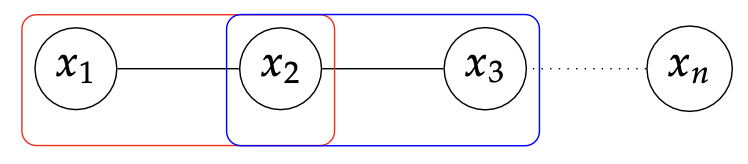
\includegraphics[width=0.7\textwidth]{assets/fig18.png}
\end{figure}

The factorization implied by this PGM is:
$$
    p(x) = \frac{1}{Z} \cdot \psi_{1,2}(x_1, x_2)\cdot \psi_{2,3}(x_2, x_3)\dots \psi_{x_{n-1}, x_{n}}(x_{n-1}, x_n)
$$

Consider now the equivalent model in case of a Bayesian Network:

\begin{center}
    \begin{tikzpicture}
        % Nodes
        \node (x1) [circle,draw] {\(\mathbf{x_1}\)};
        \node (x2) [circle,draw, right=of x1] {\(\mathbf{x_2}\)};
        \node (x3) [circle,draw, right=of x2] {\(\mathbf{x_3}\)};
        \node (xn) [circle,draw, right=of x3] {\(\mathbf{x_n}\)};
        
        % Arrows
        \draw[->] (x1) -- (x2);
        \draw[->] (x2) -- (x3);
        \draw[dotted] (x3) -- (xn);
    \end{tikzpicture}
\end{center}

The factorization in this case reads as 
$$
    p(x) = p(x_1)\cdot p(x_2|x_1)\cdot p(x_3|x_2) \dots p(x_n|x_{n-1})
$$

\begin{observationblock}[Markov processes]
    Chain structures like the previous are common because they repre-
    sent temporal series (more specifically, they are Markov processes).
\end{observationblock}

Suppose that, given the model above, we want to compute the marginal
$$
    p(x_k) = \sum_{x_1,\dots, x_{k-1},x_{k+1},x_n}^{}p(x_1,\dots, x_n)
$$

with $1<k<n$. In principle this has complexity $O(\mathcal{K}^{n-1})$.

However, plugging the factorization implied by the Markov Random Field, we get(using the distributive laws of sum and product):
$$
\begin{array}{rl}
    p(x_k)
    & = \sum_{x_-k}^{}\frac{1}{Z}\psi_{1,2}(x_1, x_2)\dots \psi_{n-1, n}(x_{n-1}, x_n)\\
    & = \frac{1}{Z} \sum_{x_{k-1}}\psi_{k-1, k}(x_{k-1}, x_k) \dots \left[ \sum_{x_2}^{}\psi_{2,3}(x_2, x_3)\left[\sum_{x_1}^{}\psi(x_1, x_2)\right]\right] + \\
    & + \sum_{x_{k+1}}^{}\psi_{k, k+1}(x_k, x_{k+1}) \dots \left[\sum_{x_{n-1}}^{}\psi_{n-2, n-1}(x_{n-2}, x_{n-1})\left[\sum_{x_n}^{}\psi_{n-1, n}(x_{n-1, x_n})\right]\right]
\end{array}
$$

Note that complexity is now $O(n\cdot k)$, i.e. linear in $n$. 

We can define a dynamic programming algorithm, called \textbf{message-passing algorithm}, in which the information from the graph is summarized by local edge information. 

We break the chain in two parts, the past and the future w.r.t. $x_k$, and we define the following:
\begin{itemize}
    \item forward message: $\mu_\alpha(x_k) = \sum_{x_{k-1}}^{}\psi_{k-1, k}(x_{k-1}, x_k)\cdot \mu_{\alpha}(x_{k-1})$, with base case $\mu_{\alpha}(x_1) = 1$
    \item backward message: $\mu_{\beta}(x_k) = \sum_{x_{k+1}}\psi_{k, k-1}(x_k, x_{k+1})\cdot \mu_{\beta}(x_{k+1})$, with base case $\mu_{\beta}(x_n) = 1$
\end{itemize}

In this algorithm, each node sends a message to its neighbors, and the messages are computed by the above formulas.

\begin{figure}[H]
    \centering
    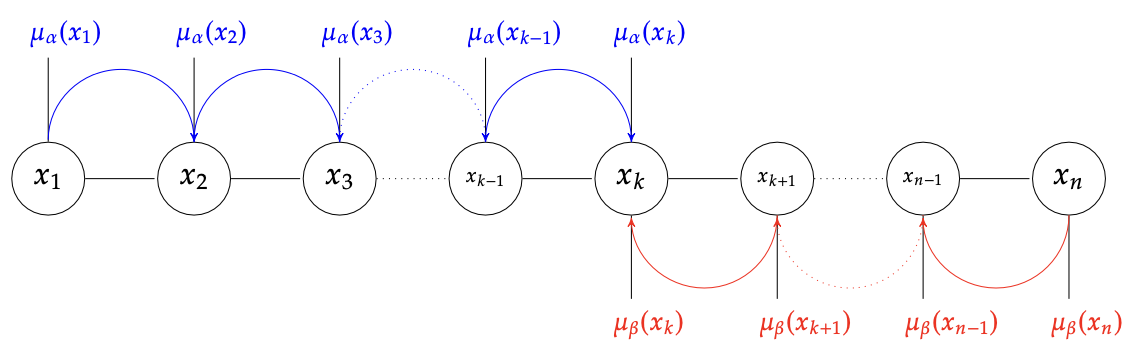
\includegraphics[width=0.9\textwidth]{assets/fig19.png}
    \caption{Message-passing algorithm}
\end{figure}

Once we have both $\mu_{\alpha}(x_k)$ and $\mu_{\beta}(x_k)$, we can observe that:
$$
    p(x_k) = \frac{1}{Z_k}\cdot \mu_{\alpha}(x_k)\mu_{\beta}(x_k) \propto \mu_{\alpha}(x_k)\mu_{\beta}(x_k)
$$
with the normalization constant $Z_k$ computed as $Z_k = \sum_{x_k}^{}\mu_{\alpha}(x_k)\mu_{\beta}(x_k)$.

Summarizing, the idea behind this algorithm is to start from the extremes of the chain and pass messages (forward and backward) until the other end is reached. Once there, messages are combined to obtain an (un)normalized marginal distribution.

\section{Factor Graphs}

Our goal in what follows is to extend what we have done for chains to more general graph structures, i.e. trees and politrees. In order to do so, we need to introduce the formalism of \textbf{Factor Graphs}.

The idea behind them is to expose in a more clear way what are the factors and what are the variables. For this reason, Factor Graphs are bipartite graphs (i.e. nodes are divided in two classes), in which we have:
\begin{table}[H]
    \centering
    \begin{tabular}{c|c}
        \textbf{Variable nodes} & \textbf{Factor nodes} \\
        \hline
        $x$ & $f$ \\

    \end{tabular}
\end{table}

The canonical way of represent bipartite graphs is the following:

\begin{center}
    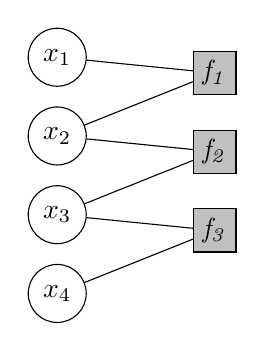
\begin{tikzpicture}
        % Nodes on the left (x variables)
        \node (x1) [circle, draw] at (0,3) {\(x_1\)};
        \node (x2) [circle, draw] at (0,2) {\(x_2\)};
        \node (x3) [circle, draw] at (0,1) {\(x_3\)};
        \node (x4) [circle, draw] at (0,0) {\(x_4\)};
        
        % Nodes on the right (f variables)
        \node (f1) [rectangle, draw, fill=gray!50] at (2,2.8) {\(\mathit{f_1}\)};
        \node (f2) [rectangle, draw, fill=gray!50] at (2,1.8) {\(\mathit{f_2}\)};
        \node (f3) [rectangle, draw, fill=gray!50] at (2,0.8) {\(\mathit{f_3}\)};
        
        % Edges
        \draw (x1) -- (f1);
        \draw (x2) -- (f1);
        \draw (x2) -- (f2);
        \draw (x3) -- (f2);
        \draw (x3) -- (f3);
        \draw (x4) -- (f3);
        
    \end{tikzpicture}
\end{center}

That is, all variable nodes are put on the left and all factor nodes on the right. 

A more convenient, equivalent, representation could be:

\begin{center}
    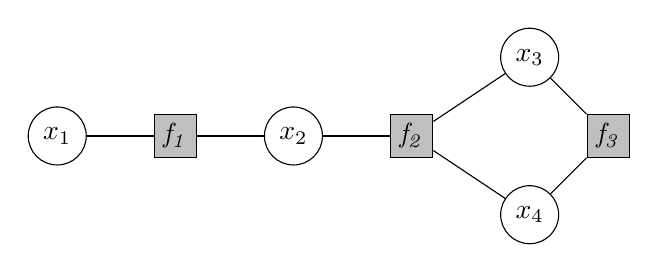
\begin{tikzpicture}
        % Nodes
        \node (x1) [circle, draw] at (0,0) {\(x_1\)};
        \node (f1) [rectangle, draw, fill=gray!50] at (1.5,0) {\(\mathit{f_1}\)};
        \node (x2) [circle, draw] at (3,0) {\(x_2\)};
        \node (f2) [rectangle, draw, fill=gray!50] at (4.5,0) {\(\mathit{f_2}\)};
        \node (x3) [circle, draw] at (6,1) {\(x_3\)};
        \node (x4) [circle, draw] at (6,-1) {\(x_4\)};
        \node (f3) [rectangle, draw, fill=gray!50] at (7,0) {\(\mathit{f_3}\)};
        
        % Edges
        \draw (x1) -- (f1);
        \draw (f1) -- (x2);
        \draw (x2) -- (f2);
        \draw (f2) -- (x3);
        \draw (f2) -- (x4);
        \draw (x3) -- (f3);
        \draw (x4) -- (f3);
    
    \end{tikzpicture}
\end{center}

\subsection{From Bayesian Networks to Factor Graphs}
Consider the following Bayesian Network:

\begin{center}
    \begin{tikzpicture}
        % Nodes
        \node (x1) [circle, draw] at (0,0) {\(x_1\)};
        \node (x2) [circle, draw] at (3,0) {\(x_2\)};
        \node (x3) [circle, draw] at (1.5,-3) {\(x_3\)};
        \node (x4) [circle, draw] at (4.5,-3) {\(x_4\)};
        \node (x5) [circle, draw] at (3,-6) {\(x_5\)};
        
        % Directed Edges
        \draw[->] (x1) -- (x3);
        \draw[->] (x2) -- (x3);
        \draw[->] (x3) -- (x5);
        \draw[->] (x4) -- (x5);
    \end{tikzpicture}
\end{center}

Which corresponds to the factorization:
$$
    \begin{array}{rl}
        p(x)
        & = p(x_1)p(x_2)p(x_3|x_1, x_2)p(x_4)p(x_5|x_3, x_4)\\
        & = f_1(x_1)f_2(x_2)f_3(x_1, x_2, x_3)f_4(x_4)f_5(x_3, x_4, x_5)
    \end{array}
$$

Fundamentally, the idea is to have a factor node (connected to the proper variable nodes) for each term of the factorization implied by the Bayesian Network.

Formally: $\forall p(x_j|pa_j) \to f_j \curvearrowright {x_j} \cup pa_j$.

Hence the Factor Graph equivalent to the Bayesian Network above is:

\begin{center}
    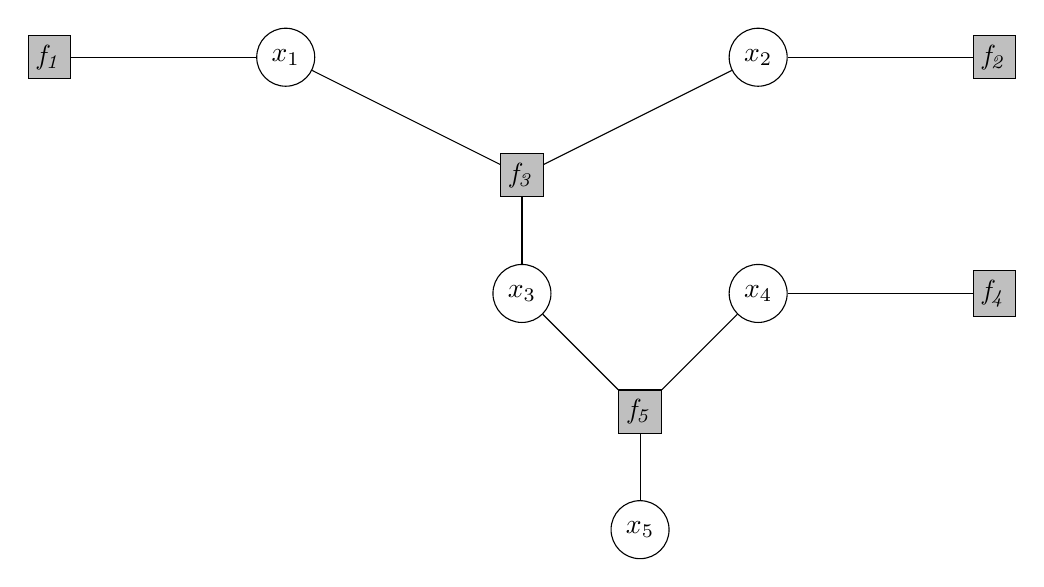
\begin{tikzpicture}
        % Nodes
        \node (x1) [circle, draw] at (0,0) {\(x_1\)};
        \node (f1) [rectangle, draw, fill=gray!50] at (-3,0) {\(\mathit{f_1}\)};
        \node (x2) [circle, draw] at (6,0) {\(x_2\)};
        \node (f2) [rectangle, draw, fill=gray!50] at (9, 0) {\(\mathit{f_2}\)};
        \node (x3) [circle, draw] at (3, -3) {\(x_3\)};
        \node (f3) [rectangle, draw, fill=gray!50] at (3, -1.5) {\(\mathit{f_3}\)};
        \node (x4) [circle, draw] at (6, -3) {\(x_4\)};
        \node (f4) [rectangle, draw, fill=gray!50] at (9, -3) {\(\mathit{f_4}\)};
        \node (x5) [circle, draw] at (4.5, -6) {\(x_5\)};
        \node (f5) [rectangle, draw, fill=gray!50] at (4.5, -4.5) {\(\mathit{f_5}\)};
        
        % Edges
        \draw (x1) -- (f1);
        \draw (x1) -- (f3);
        \draw (x2) -- (f3);
        \draw (x2) -- (f2);
        \draw (x3) -- (f3);
        \draw (x3) -- (f5);
        \draw (x4) -- (f4);
        \draw (x4) -- (f5);
        \draw (x5) -- (f5);
    
    \end{tikzpicture}
\end{center}

\subsection{From Markov Random Fields to Factor Graphs}
Consider the following Markov Random Field (rectangles correspond to the cliques):
\begin{figure}[H]
    \centering
    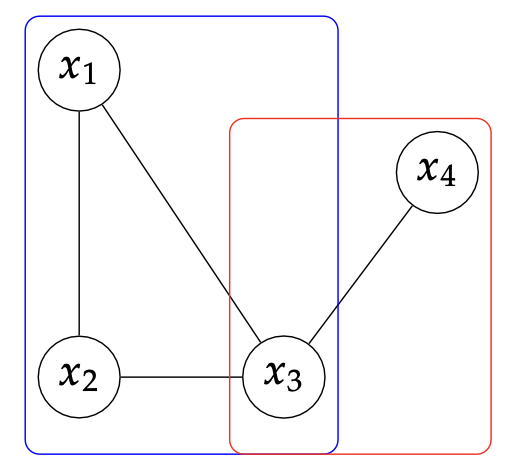
\includegraphics[width=0.5\textwidth]{assets/fig20.png}
\end{figure}

Which implies the factorization:
$$
    p(x) = \frac{1}{Z}\psi_1(x_1, x_2, x_3)\psi_2(x_3, x_4) = \frac{1}{Z}f_1(x_1, x_2, x_3)f_2(x_3, x_4)
$$

This leads to the following Factor Graph:
\begin{center}
    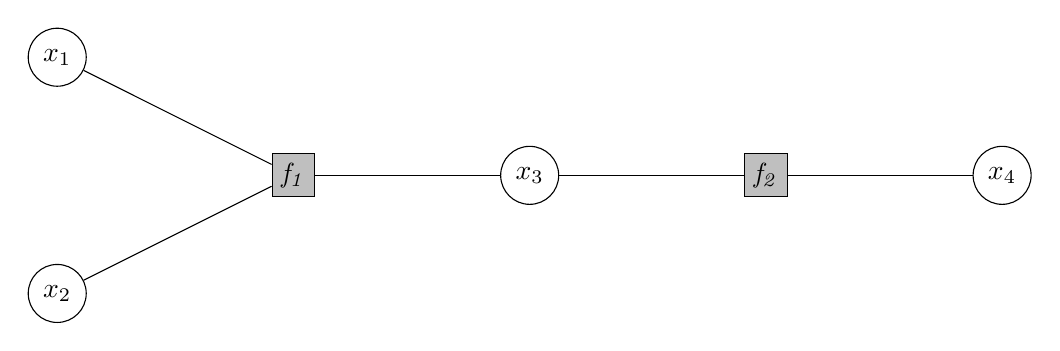
\begin{tikzpicture}
        % Nodes
        \node (x1) [circle, draw] at (-3, 1.5) {\(x_1\)};
        \node (f1) [rectangle, draw, fill=gray!50] at (0,0) {\(\mathit{f_1}\)};
        \node (x2) [circle, draw] at (-3, -1.5) {\(x_2\)};
        \node (f2) [rectangle, draw, fill=gray!50] at (6,0) {\(\mathit{f_2}\)};
        \node (x3) [circle, draw] at (3, 0) {\(x_3\)};
        \node (x4) [circle, draw] at (9, 0) {\(x_4\)};
        
        % Edges
        \draw (x1) -- (f1);
        \draw (f1) -- (x2);
        \draw (f1) -- (x3);
        \draw (f2) -- (x4);
        \draw (x3) -- (f2);
    
    \end{tikzpicture}
\end{center}

Hence, the conversion from Markov Random Fields to Factor Graphs works as: $\forall c \in \mathcal{C} \rightarrow f_c(x_c) \sim \psi_c(x_c) $ (equality does not hold because of
the normalization constant).

So, whether we are starting from a Bayesian Network or from a Markov
Random Field, we can convert our PGM into a Factor Graph and perform
message passing on it, without loss of generality.

\section{Sum Product Algotithm}

Our goal is now to do inference in Factor Graphs, generalizing to more
general graph structures what we did with chains previously. Consider
the following Factor Graph:


\begin{center}
    \begin{tikzpicture}
        % Nodes
        \node(x1) [circle, draw] at (-6, 1.5) {\(x_1\)};
        \node (f1) [rectangle, draw, fill=gray!50] at (-3,1.5) {\(\mathit{f_1}\)};
        \node (x2) [circle, draw] at (-6, -1.5) {\(x_2\)};
        \node (f2) [rectangle, draw, fill=gray!50] at (-3,-1.5) {\(\mathit{f_2}\)};
        \node (x3) [circle, draw] at (0, 0) {\(x_3\)};
        \node (f3) [rectangle, draw, fill=gray!50] at (3, -1.5) {\(\mathit{f_3}\)};
        \node (x4) [circle, draw] at (0, -3) {\(x_4\)};
        \node (x5) [circle, draw] at (6, -1.5) {\(x_5\)};
    
        % Edges
        \draw (x1) -- (f1);
        \draw (f1) -- (x3);
        
        \draw (x2) -- (f2);
        \draw (f2) -- (x3);
        
        \draw (x3) -- (f3);
        \draw (x4) -- (f3);
        
        \draw (f3) -- (x5);
    
        % Labels
        \node[left=of x1, blue] {leaf};
        \node[left=of x2, blue] {leaf};
        \node[left=of x4, blue] {leaf};
        \node[right=of x5, red] {root};
    
    \end{tikzpicture}
    \end{center}

The joint probabbility distribution implied by thie Factor Graph is:
$$
p(x) = f_1(x_1, x_3)f_2(x_2, x_3)f_3(x_3, x_4, x_5)
$$


